\chapter{Introduzione}
\section{Premessa}
La seguente relazione idraulica si pone lo scopo di progettare e dimensionare una rete di drenaggio urbano delle acque meteoriche del quartiere "Le Albere" a Sud-Ovest del centro storico di Trento (Figura \ref{fig:inquadramentoGenerale}), cercando inoltre di attenuare e ritardare il picco di piena.

%Come prima cosa si è fatto un inquadramento generale della zona tramite il software GIS OpenSource QGIS, in cui si è svolta un valutazione della zona con suddivisione in sottobacini, individuazione di lunghezze di drenaggio, superfici impermeabili e pendenze medie, come spiegato nel prossimo {\RED{paragrafo}}.

Come prima cosa si è fatto un inquadramento generale della zona tramite il software GIS OpenSource QGIS, in cui si è svolta una preliminare valutazione idrologica del terreno, come spiegato più approfonditamente nel prossimo paragrafo.

%Per ottenere il massimo risultato dalla rete si è svolto prima di tutto un inquadramento dell'area di studio andando a studiarne le caratteristiche pluviometriche. 

%Dopodiché si è eseguita l'analisi idrologica e idraulica dall'area allo stato di fatto per poi passare alla rete di smaltimento delle acque allo stato di progetto, esaminando il comportamento della rete con la presenza di sistemi di laminazione puntuali, come le vasche volano, e sistemi diffusi, come i LID.

%Nel capitolo \ref{cap:pluviometriche} si vedrà lo studio idrologico dell'area attraverso il calcolo dei parametri delle curve di possibilità pluviometriche dalle elaborazioni della stazione meteorologica delle Laste (TN), successivamente nel capitolo \ref{cap:progettoBase} si vedrà come saranno utilizzati per analizzare la situazione idrologica e idraulica della zona. A tale scopo si utilizza il software Storm Water Management Model (SWMM) prodotto dall'US-EPA.

Nel capitolo \ref{cap:pluviometriche} si otterranno i parametri delle curve di possibilità pluviometriche dalle elaborazioni della stazione meteorologica delle Laste (TN), successivamente nel capitolo \ref{cap:progettoBase} si vedrà come saranno utilizzati per analizzare la situazione idrologica e idraulica della zona. A tale scopo si utilizza il software Storm Water Management Model (SWMM) prodotto dall'US-EPA.

A questo punto verrà progettata e verificata, nel capitolo \ref{cap:ProgettoRete}, una rete di drenaggio delle acque meteoriche. Si valuterà il riempimento e la portata massima uscente per poi attenuarla attraverso l'aggiunta alla rete di sistemi di laminazione puntuali e diffusi.

Nell'ultimo paragrafo si effettuerà una stima dei costi di costruzione delle opere progettate.


%%%%%%%
\section{Valutazione dell’area di studio in QGIS}
\subsection{Inquadramento dell'area di studio}
\begin{figure}[p]
    \centering
    \includegraphics[trim=0cm 0cm 0cm 0cm,clip,frame,width=0.9\textwidth]{IMG/Inquadramento_Generale_scala1-10000.pdf} 
    \caption{Inquadramento dell'area di studio all'interno della città di Trento -- Scala 1:10\,000}
    \label{fig:inquadramentoGenerale}
\end{figure}
\begin{figure}[p]
    \centering
    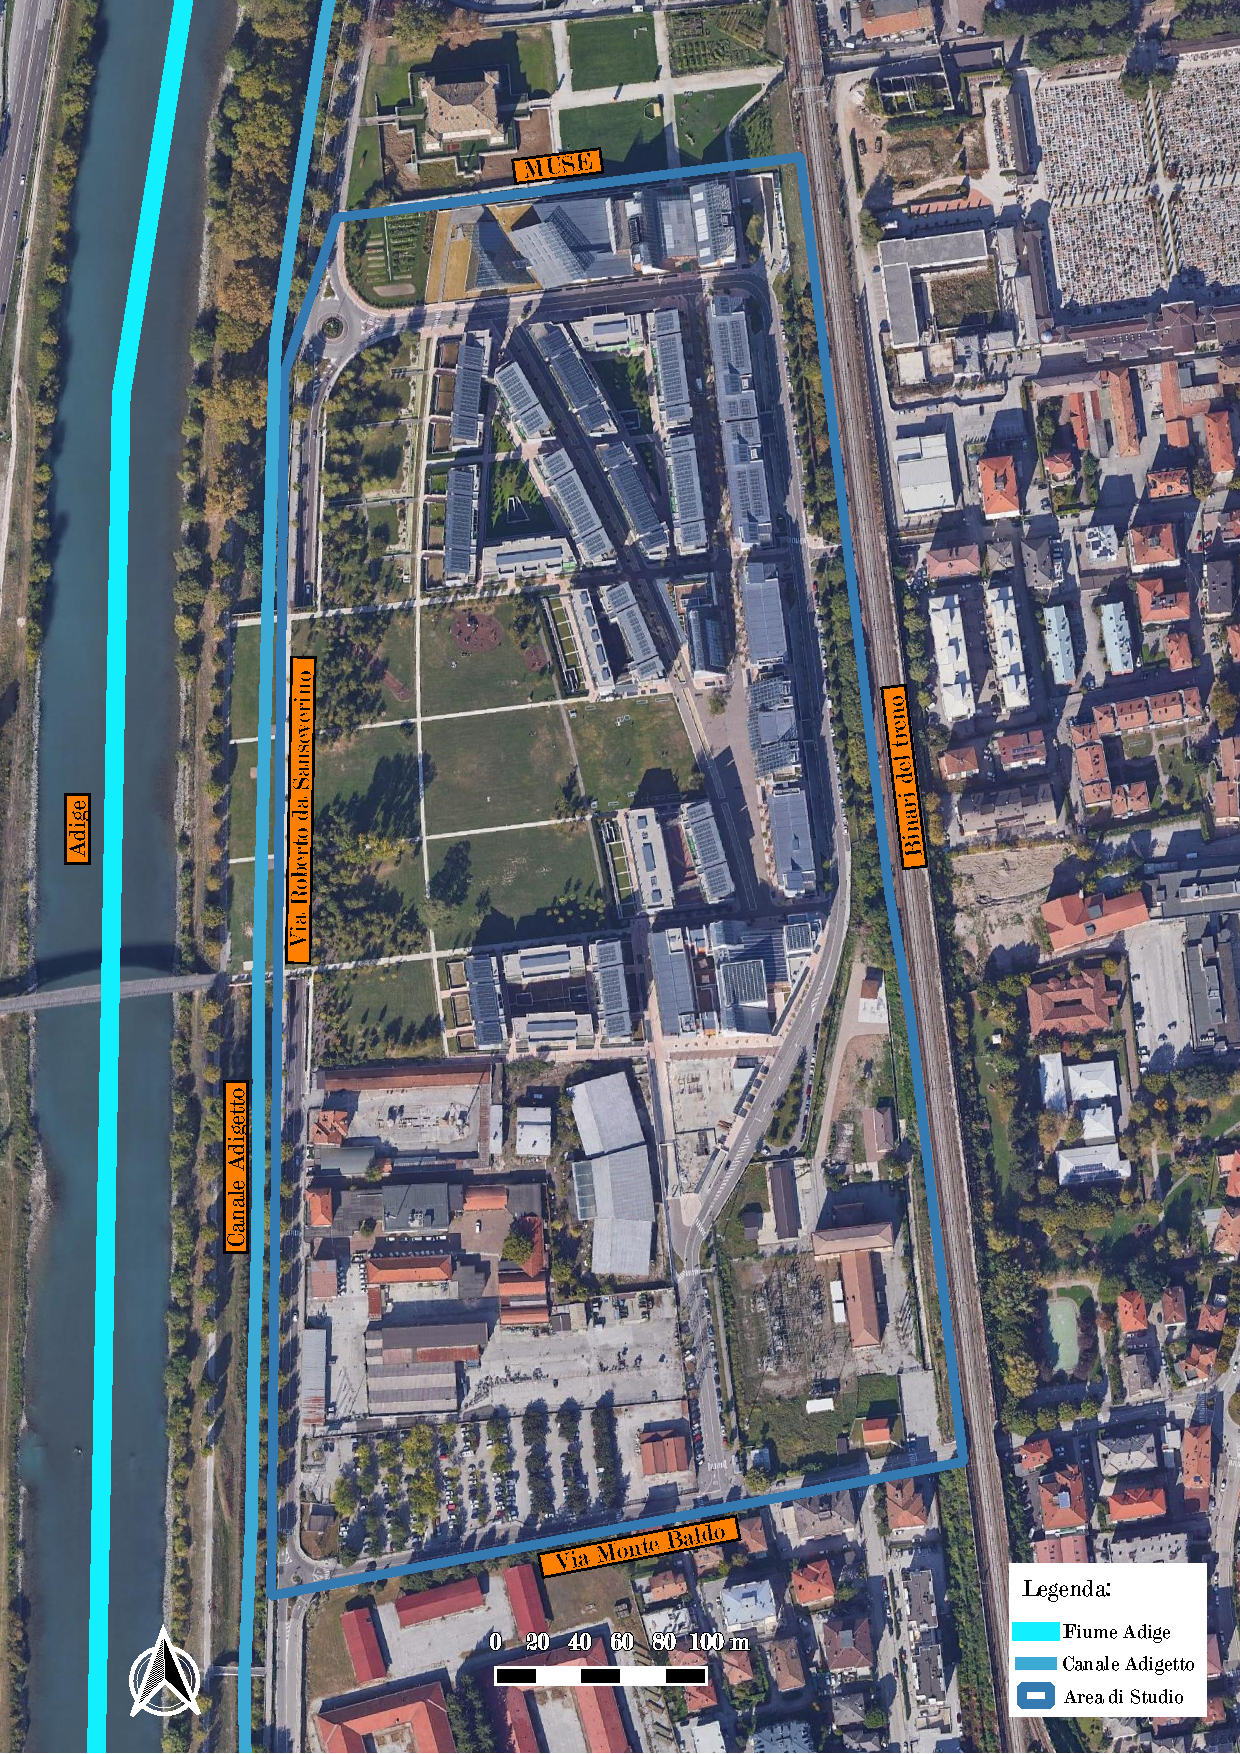
\includegraphics[trim=0cm 0cm 0cm 0cm,clip,frame,width=0.9\textwidth]{IMG/Inquadramento_scala1-2800.pdf} 
    \caption{Delimitazioni viarie e fluviali dell'area di studio -- Scala 1:2\,800}
    \label{fig:inquadramentoDettaglio}
\end{figure}

Per ottenere un ottimale inquadramento della zona si fa uso del programma QGIS sul quale dopo aver caricato le opportune mappe e aver impostato il corretto sistema di riferimento delle coordinate che, essendo l'area di studio a Trento, risulta essere WGS 84/UTM zone 32N con ID dell'autorità EPSG:32632.
Una volta immessi i dati generali su QGIS si prosegue con l'inquadramento del bacino urbano di studio.

%L'area di studio nella quale si svolge il dimensionamento della rete di drenaggio delle acque meteoriche si identifica come quartiere "Le Albere" a Sud-Ovest del centro storico di Trento (Figura \ref{fig:inquadramentoGenerale}).
La zona in esame è compresa a nord e sud tra il MUSE e Via Monte Baldo, mentre ad est ed ovest rispettivamente tra i binari del treno, linea Brennero-Verona, e Via Roberto da Sanseverino (Figura \ref{fig:inquadramentoDettaglio}).
L'area si espande per un totale di circa \SI{185000}{\square\metre} e il piano campagna è compreso tra una quota di \SI{187} e \SI{194.5}{\metre\,s.l.m.}. 

Come si evince dalla figura \ref{fig:inquadramentoDettaglio} l'aria di studio è posizionata in vicinanza del fiume Adige e del canale Adigetto; fiume in cui si posizioneranno i tre recapiti finali della rete di drenaggio progettata rispettivamente a nord, al centro e a sud di via Roberto da Sanseverino.

\subsection{Sottobacini}
%Prima di procedere sul software SWMM si eseguono alcuni passaggi iniziali su QGIS. 
%%Dopo aver eseguito un primo inquadramento della zona si proseguono le operazioni iniziali per impostare la successiva analisi idrologica e idraulica dall'area.

In questa prima fase progettuale per eseguire un'analisi più precisa si è discretizzata l'area di progetto in una ventina di sottobacini. 
Questa ripartizione si svolge per ottenere un'analisi del deflusso migliore sull'area di studio (Figura \ref{fig:sottobacini}).

\begin{figure}[p]
    \centering
    \includegraphics[trim=0cm 0cm 0cm 0cm,clip,frame,width=0.9\textwidth]{IMG/sottobacini.pdf} 
    \caption{Suddivisione dell'area di studio in diversi sottobacini}
    \label{fig:sottobacini}
\end{figure}

In ciascuna suddivisione, con l'aiuto delle curve di livello, che permettono di capire la pendenza del terreno e il lato del sottobacino in cui le acque defluiscono, si realizzano le lunghezze di drenaggio. 
Queste ultime si cercano di costruirle a una distanza standard e il più perpendicolare possibile alle curve di livello.
Si determinano circa quattro lunghezze di drenaggio per sottobacino.

In seguito si ricavano e valutano i principali dati per lo svolgimento dell'analisi tra cui la pendenza media, le aree totali e le superfici impermeabili per ogni sottobacino, utili per l'analisi del drenaggio in SWMM e la successiva progettazione della rete.

%Infine si ipotizza una rete di drenaggio con l'individuazione dei nodi e delle condotte da inserire successivamente sul programma SWMM.
%%%%%%%
